\documentclass[UTF8,zihao=-4,a4paper,fontset=none]{ctexart}

\usepackage{geometry}
\geometry{
  a4paper,
  left=2.8cm,
  right=2.2cm,
  top=2.8cm,
  bottom=2.5cm,
  headheight=16pt,
  headsep=0.5cm,
  footskip=1.2cm
}

\usepackage{amsmath,amssymb}
\usepackage{array}
\usepackage{fancyhdr}
\usepackage{fontspec}
\usepackage{graphicx}
\usepackage[hypertexnames=false]{hyperref}
\usepackage{indentfirst}
\usepackage{listings}
\usepackage{pdfpages}
\usepackage{setspace}
\usepackage{xcolor}

\hypersetup{
  hidelinks,
  pdfencoding=auto,
  pdftitle={中国人民公安大学本科毕业论文（设计）},
  pdfauthor={学生姓名}
}
\pdfstringdefDisableCommands{\def\quad{ }}

\IfFontExistsTF{Times New Roman}{\setmainfont{Times New Roman}}{}
\setCJKmainfont{SIMSUN.TTC}[Path=fonts/,AutoFakeBold=3,AutoFakeSlant=.2]
\setCJKsansfont{SIMHEI.TTF}[Path=fonts/,AutoFakeBold=3,AutoFakeSlant=.2]
\setCJKmonofont{SIMSUN.TTC}[Path=fonts/,AutoFakeBold=3,AutoFakeSlant=.2]
\setCJKfamilyfont{coverkai}{楷体_GB2312.TTF}[Path=fonts/,AutoFakeBold=3,AutoFakeSlant=.2]
\setCJKfamilyfont{coverfang}{仿宋_GB2312.TTF}[Path=fonts/,AutoFakeBold=3,AutoFakeSlant=.2]
\setCJKfamilyfont{zhsong}{SIMSUN.TTC}[Path=fonts/,AutoFakeBold=3,AutoFakeSlant=.2]
\setCJKfamilyfont{zhhei}{SIMHEI.TTF}[Path=fonts/,AutoFakeBold=3,AutoFakeSlant=.2]
\setCJKfamilyfont{zhkai}{楷体_GB2312.TTF}[Path=fonts/,AutoFakeBold=3,AutoFakeSlant=.2]
\setCJKfamilyfont{zhfs}{仿宋_GB2312.TTF}[Path=fonts/,AutoFakeBold=3,AutoFakeSlant=.2]
\providecommand{\songti}{\CJKfamily{zhsong}}
\providecommand{\heiti}{\CJKfamily{zhhei}}
\providecommand{\kaishu}{\CJKfamily{zhkai}}
\providecommand{\fangsong}{\CJKfamily{zhfs}}

\newcommand{\coverkai}{\CJKfamily{coverkai}}
\newcommand{\coverfang}{\CJKfamily{coverfang}}
\newcommand{\bodyplaceholder}{［单击此处键入内容］}
\newcommand{\coverfillc}[2]{\underline{\makebox[#1][c]{#2}}}

\setstretch{1.3}
\setlength{\parindent}{0pt}
\urlstyle{same}

\lstset{
  basicstyle=\ttfamily\fontsize{7.5pt}{9pt}\selectfont,
  keywordstyle=\color{black},
  commentstyle=\color{black!60},
  stringstyle=\color{black},
  numbers=left,
  numberstyle=\ttfamily\fontsize{7pt}{8pt}\selectfont\color{black!65},
  stepnumber=1,
  numbersep=7pt,
  frame=single,
  framerule=0.25pt,
  rulecolor=\color{black!15},
  backgroundcolor=\color{black!3},
  breaklines=false,
  showstringspaces=false,
  tabsize=4,
  keepspaces=true,
  columns=fullflexible,
  xleftmargin=0.8em,
  xrightmargin=0.2em,
  framexleftmargin=0.7em,
  framesep=4pt,
  aboveskip=0.15cm,
  belowskip=0pt
}

\fancypagestyle{thesisstyle}{
  \fancyhf{}
  \fancyhead[C]{\songti\zihao{5} 中国人民公安大学本科毕业论文（设计）}
  \fancyfoot[C]{\songti\zihao{5}\thepage}
  \renewcommand{\headrulewidth}{0.4pt}
  \renewcommand{\footrulewidth}{0pt}
}
\fancypagestyle{plain}{
  \fancyhf{}
  \fancyhead[C]{\songti\zihao{5} 中国人民公安大学本科毕业论文（设计）}
  \fancyfoot[C]{\songti\zihao{5}\thepage}
  \renewcommand{\headrulewidth}{0.4pt}
  \renewcommand{\footrulewidth}{0pt}
}

\newcommand{\thesistitlecn}{［键入论文题目］}
\newcommand{\thesissubtitlecn}{［键入论文副标题或删除此行］}
\newcommand{\cnabstracttitle}{［单击此处键入标题］}
\newcommand{\cnabstractsubtitle}{［单击此处继续键入副标题或删除此行］}
\newcommand{\thesistitleen}{［单击此处键入英文标题］}
\newcommand{\thesissubtitleen}{［单击此处继续键入英文副标题或删除此行］}
\newcommand{\studentname}{［键入学生姓名］}
\newcommand{\studentid}{［键入学号］}
\newcommand{\college}{［键入学院名称］}
\newcommand{\grade}{［键入年级］}
\newcommand{\major}{［键入专业名称］}
\newcommand{\company}{［键入区队］}
\newcommand{\advisor}{［键入指导教师姓名］}
\newcommand{\cnabstracttext}{［中文摘要内容一般为 200-300 字左右，五号，仿宋］}
\newcommand{\cnkeywordslineone}{［五号，仿宋］；［单击此处键入关键词］；［单击此处键入关键词］；［单击此处键入关键词或删除］；}
\newcommand{\cnkeywordslinetwo}{［单击此处键入关键词或删除］；［单击此处键入关键词或删除］；［单击此处键入关键词或删除］；［单击此处键入关键词或删除］}
\newcommand{\enabstracttext}{［单击此处键入英文摘要内容，与中文摘要相对应，一般不宜超过 250 个实词］}
\newcommand{\enkeywordslineone}{［单击此处键入关键词］；［单击此处键入关键词］；［单击此处键入关键词］；［单击此处键入关键词或删除］；}
\newcommand{\enkeywordslinetwo}{［单击此处键入关键词或删除］；［单击此处键入关键词或删除］；［单击此处键入关键词或删除］；［单击此处键入关键词或删除］}
\newcommand{\conclusiontext}{［单击此处键入内容］}
\newcommand{\acknowledgementtext}{［单击此处键入致谢词］}
\newcommand{\referencetitle}{参考文献}
\newcommand{\referenceentryone}{[1] [序号] 主要责任者. 题名[文献类型标识]. 其他责任者. 版本项. 出版地: 出版者, 出版年: 引文页码[引用日期]. 获取和访问路径.}
\newcommand{\referenceentrytwo}{[2] [序号] 析出文献主要责任者. 析出文献题名[文献类型标识]//专著主要责任者. 专著题名. 出版地: 出版者, 版年: 析出文献的页码[引用日期].}
\newcommand{\referenceentrythree}{[3] [序号] 析出文献主要责任者. 析出文献题名[文献类型标识]. 期刊题名, 年, 卷(期): 页码.}
\newcommand{\referenceentryfour}{[4] [序号] 析出文献主要责任者. 析出文献题名[文献类型标识]. 报纸题名, 年-月-日(版次).}
\newcommand{\referenceentryfive}{[5] [序号] 专利申请者或所有者. 专利题名: 专利号[文献类型标识]. 公告日期或公开日期. 获取和访问路径.}
\newcommand{\referenceentrysix}{[6] [序号] 主要责任者. 题名[文献类型标识/文献载体标识]. (发布日期)[引用日期]. 获取和访问路径.}
\newcommand{\referenceentryseven}{[7] [序号] 主要责任者. 题名[文献类型标识/文献载体标识]. 出版地: 出版者, 出版年[引用日期]. 获取和访问路径.}
\newcommand{\referenceentryeight}{[8] [序号] 主要责任者. 题名[文献类型标识/文献载体标识]. 连续出版物题名, 年, 卷(期): 页码[引用日期]. 获取和访问路径.}
\newcommand{\referenceentrynine}{[9] [序号] 主要责任者. 文献题名[Z]. 出版地: 出版者, 出版年.}
\newcommand{\referenceentryten}{}
\newcommand{\appendixtitle}{附\quad 录}
\newcommand{\appendixnote}{（信网统一格式，供参考）}
\newcommand{\appendixatitle}{附录A:图目录}
\newcommand{\appendixbtitle}{附录B:表目录}

\newcommand{\dotleaders}{\nobreak\leaders\hbox to 0.45em{\hss.\hss}\hfill\nobreak}
\newcommand{\appendixline}[2]{\noindent #1\dotleaders #2\par}
\newcommand{\insertofficialpage}[1]{
\includepdf[pages={#1},fitpaper=true,pagecommand={\thispagestyle{empty}}]{assets/official-template.pdf}}
\newcommand{\manualtitle}[1]{\begin{center}{\heiti\zihao{3}#1\par}\end{center}}
\newcommand{\manualsubsection}[1]{{\heiti\zihao{4}#1\par}}
\newcommand{\manualsubsubsection}[1]{{\heiti\zihao{-4}#1\par}}
\newcommand{\manualparagraph}[1]{{\songti\zihao{-4}#1\par}}

\newcommand{\makethesistitlepage}{
  \begin{titlepage}
    \thispagestyle{empty}
    \centering
    \vspace*{1.05cm}
    
\includegraphics[width=9.5cm]{assets/pup-title.png}\par
    \vspace{0.85cm}
    {\coverkai\bfseries\fontsize{29bp}{31bp}\selectfont 毕业论文（设计）\par}
    \vspace{0.7cm}
    
\includegraphics[width=3.7cm]{assets/pup-emblem-gray.png}\par
    \vspace{1.35cm}

    {\heiti\zihao{-3}题目：\coverfillc{7.6cm}{\thesistitlecn}\par}
    \vspace{0.55cm}
    {\zihao{4}--\ \coverfillc{6.9cm}{\thesissubtitlecn}\par}
    \vspace{0.95cm}

    {\renewcommand{\arraystretch}{2.0}
    \begin{tabular}{@{}p{1.9cm}p{3.8cm}p{1.55cm}p{2.7cm}@{}}
      \heiti 姓名： & \coverfillc{3.3cm}{\studentname} & \heiti 学号： & \coverfillc{2.45cm}{\studentid} \\
      \heiti 学院： & \coverfillc{3.3cm}{\college} & \heiti 年级： & \coverfillc{2.45cm}{\grade} \\
      \heiti 专业： & \coverfillc{3.3cm}{\major} & \heiti 区队： & \coverfillc{2.45cm}{\company} \\
      \multicolumn{4}{c}{\heiti 指导教师：\coverfillc{6.0cm}{\advisor}}
    \end{tabular}\par}

    \vfill
    {\coverfang\bfseries\zihao{-3} 教\ 务\ 处\ 制\par}
  \end{titlepage}
}

\newcommand{\makecnabstractpage}{
  \clearpage
  \pagestyle{thesisstyle}
  \pagenumbering{Roman}
  \setcounter{page}{1}
  \vspace*{0.45cm}
  \begin{center}
    {\heiti\zihao{-2}\cnabstracttitle\par}
    \vspace{0.18cm}
    {\zihao{4}--\ [\cnabstractsubtitle]\par}
  \end{center}
  \vspace{0.8cm}
  {\begingroup
  \coverfang\zihao{5}\selectfont
  \setstretch{1.2}
  \noindent\makebox[5.6em][l]{\heiti 摘\quad 要：}\parbox[t]{0.8\textwidth}{\cnabstracttext}\par
  \vspace{0.45cm}
  \noindent\makebox[5.6em][l]{\heiti 关\ 键\ 词：}\parbox[t]{0.8\textwidth}{\cnkeywordslineone\par \cnkeywordslinetwo}\par
  \endgroup}
}

\newcommand{\makeenabstractpage}{
  \clearpage
  \pagestyle{thesisstyle}
  \vspace*{0.45cm}
  \begin{center}
    {\bfseries\zihao{-2}\thesistitleen\par}
    \vspace{0.18cm}
    {\zihao{4}--\ [\thesissubtitleen]\par}
  \end{center}
  \vspace{0.8cm}
  {\begingroup
  \zihao{5}\selectfont
  \setstretch{1.2}
  \noindent\makebox[6.2em][l]{\bfseries Abstract:}\parbox[t]{0.77\textwidth}{\enabstracttext}\par
  \vspace{0.45cm}
  \noindent\makebox[6.2em][l]{\bfseries Keywords:}\parbox[t]{0.77\textwidth}{\enkeywordslineone\par \enkeywordslinetwo}\par
  \endgroup}
}

\begin{document}

\insertofficialpage{1}
\insertofficialpage{2}
\insertofficialpage{3}
\insertofficialpage{4}
\insertofficialpage{5}

\clearpage
\pagenumbering{arabic}
\setcounter{page}{1}
\pagestyle{thesisstyle}
\vspace*{0.55cm}
\manualtitle{1.引\quad 言}
\vspace{0.55cm}
{\songti\zihao{-4}\bodyplaceholder\par}

\vspace{1.25cm}
\manualtitle{2.【单击此处键入一级标题】}
\vspace{0.6cm}
\manualsubsection{2.1【单击此处键入二级标题】}
\vspace{0.2cm}
\manualsubsubsection{2.1.1［单击此处键入内容］}
\vspace{0.12cm}
\manualparagraph{2.1.1.1［单击此处键入内容］}

\vspace{0.55cm}
\manualsubsection{2.2【单击此处键入二级标题】}
\vspace{0.2cm}
{\songti\zihao{-4}\bodyplaceholder\par}

\vspace{1.0cm}
\manualtitle{3.【单击此处键入一级标题】}
\vspace{0.6cm}
\manualsubsection{3.1【单击此处键入二级标题】}
\vspace{0.2cm}
{\songti\zihao{-4}\bodyplaceholder\par}

\vspace{1.0cm}
{\heiti\zihao{-4}公式使用示例（信网统一格式，供参考）：\par}
{\songti\zihao{-4}公式使用公式编辑器\par}
{\songti\zihao{-4}示例 1:\par}
\vspace{0.1cm}
\begin{equation}
  \begin{aligned}
    W(N_1) &= H_{0,1} + \int_{-\tau}^{-1+1/\tau} L_{\alpha}r e^{-2\pi i\alpha N_1}\,d\alpha \\
           &= R(N_0) + \int_{-\tau}^{-1+1/\tau} L_{\alpha}r e^{-2\pi i\alpha N_1}\,d\alpha + O(P_r^{-n-v})
  \end{aligned}
  \tag{1}
\end{equation}

\clearpage
\pagestyle{thesisstyle}
\vspace*{0.1cm}
{\songti\zihao{-4}示例 2:\par}
\vspace{0.05cm}
\begin{equation}
  \begin{aligned}
    f(x,y) &= f(0,0) + \frac{1}{1!}\left(x\frac{\partial}{\partial x} + y\frac{\partial}{\partial y}\right)f(0,0) \\
           &\quad + \frac{1}{2!}\left(x\frac{\partial}{\partial x} + y\frac{\partial}{\partial y}\right)^2 f(0,0) + \cdots \\
           &\quad + \frac{1}{n!}\left(x\frac{\partial}{\partial x} + y\frac{\partial}{\partial y}\right)^n f(0,0) + \cdots
  \end{aligned}
  \tag{2}
\end{equation}

\vspace{0.35cm}
{\heiti\zihao{-4}表格使用示例（信网统一格式，供参考）：\par}
{\songti\zihao{-4}表题用五号宋体，在表上居中排，表内字体为宋体，字号可根据需要选择。\par}
{\songti\zihao{-4}示例 1:\par}
\vspace{0.2cm}
\begin{center}
  {\songti\zihao{5}表 1\quad 文献类型和标识代码\par}
  \vspace{0.1cm}
  {\songti\zihao{5}
  \setlength{\tabcolsep}{18pt}
  \renewcommand{\arraystretch}{1.18}
  \begin{tabular}{>{\centering\arraybackslash}p{5.0cm}|>{\centering\arraybackslash}p{2.8cm}}
    \hline
    文献类型 & 标识代码 \\
    \hline
    普通图书 & M \\
    会议录、论文集 & C \\
    汇编 & G \\
    报纸 & N \\
    期刊 & J \\
    学位论文 & D \\
    报告 & R \\
    标准 & S \\
    专利 & P \\
    数据库 & DB \\
    计算机程序 & CP \\
    电子公告 & EB \\
    档案 & A \\
    舆图 & CM \\
    数据集 & DS \\
    其他 & Z \\
    \hline
  \end{tabular}\par}
\end{center}

\vspace{0.15cm}
\begin{center}
  {\songti\zihao{5}表 2\quad 电子资源载体和标识代码\par}
  \vspace{0.1cm}
  {\songti\zihao{5}
  \setlength{\tabcolsep}{18pt}
  \renewcommand{\arraystretch}{1.18}
  \begin{tabular}{>{\centering\arraybackslash}p{5.0cm}|>{\centering\arraybackslash}p{2.8cm}}
    \hline
    电子资源载体类型 & 载体类型标识代码 \\
    \hline
    磁带(magnetic tape) & MT \\
    磁盘(disk) & DK \\
    \hline
  \end{tabular}\par}
\end{center}

\clearpage
\pagestyle{thesisstyle}
\vspace*{0.05cm}
\begin{center}
  {\songti\zihao{5}
  \setlength{\tabcolsep}{18pt}
  \renewcommand{\arraystretch}{1.18}
  \begin{tabular}{>{\centering\arraybackslash}p{5.0cm}|>{\centering\arraybackslash}p{2.8cm}}
    \hline
    光盘(CD-ROM) & CD \\
    联机网络(online) & OL \\
    \hline
  \end{tabular}\par}
\end{center}

\vspace{0.55cm}
{\heiti\zihao{-4}图的使用示例（信网统一格式，供参考）：\par}
{\songti\zihao{-4}文中图按先后顺序统一编号，序号用阿拉伯数字表示，如图等。每一图都应有简短确切的题名，图题在图的正下方，居中。图尽量不要使用深色背景。\par}
\vspace{0.25cm}
\begin{center}
  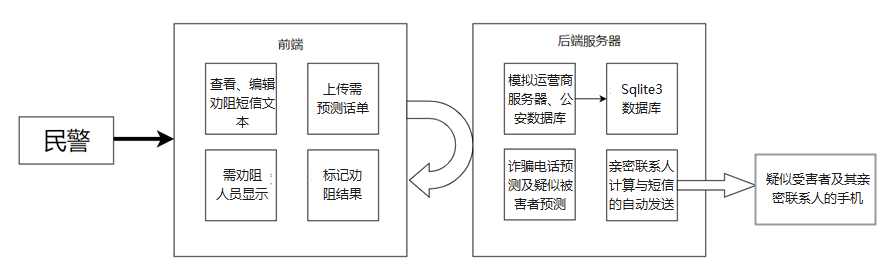
\includegraphics[width=0.86\textwidth]{assets/sample-framework.png}\par
  \vspace{0.12cm}
  {\songti\zihao{5}图 2\quad web 控制平台整体框架图}
\end{center}

\vspace{0.35cm}
{\heiti\zihao{-4}代码的使用示例（信网统一格式，供参考）：\par}
\vspace{0.18cm}
{\songti\zihao{-4}代码如下：\par}
\vspace{0.08cm}
\begin{lstlisting}
for line in open("词频统计(总).txt", encoding='utf-8'):#打开目标文件
    arr = line.split(" ")#按行分割
    frequencies[arr[0]] = float(arr[1])#将词频写入字典
wcloud = wordcloud.WordCloud(width=1000, height=700, background_color='white',
font_path='msyh.ttc')#生成词云对象
wcloud.generate_from_frequencies(frequencies)#将词频导入词云中
plt.imshow(wcloud)#接受词云图像
plt.axis('off')#关闭坐标系
plt.show()#显示词云对象
\end{lstlisting}

\insertofficialpage{9}
\insertofficialpage{10}
\insertofficialpage{11}
\insertofficialpage{12}

\end{document}
